\documentclass[11pt,a4paper]{article}
% Společné nastavení pro protokoly KI/PZS (pdfLaTeX, Overleaf výchozí kompilátor)
\usepackage[utf8]{inputenc}
\usepackage[T1]{fontenc}
\usepackage[czech]{babel}
\usepackage{lmodern}
\usepackage{amsmath}
\usepackage[a4paper,margin=2.5cm]{geometry}
\usepackage{microtype}
\usepackage{graphicx}
\usepackage{booktabs}
\usepackage{array}
\usepackage{tabularx}
\usepackage{xcolor}
\usepackage{enumitem}
\usepackage[font=small,labelfont=bf]{caption}
\usepackage{subcaption}
\usepackage{float}
\usepackage{tikz}
\usetikzlibrary{arrows.meta,positioning,shapes.geometric,calc}
\usepackage{pgfplots}
\pgfplotsset{compat=1.17}
\usepackage[hidelinks]{hyperref}

\setlist{itemsep=2pt,topsep=4pt}
\setlength{\parindent}{0pt}
\setlength{\parskip}{6pt}

% Záporné znaménko v textových tabulkách: \m0,5 -> −0,5
\newcommand{\m}{$-$}

% Červená značka pro místa, která je třeba před odevzdáním doplnit
\newcommand{\doplnit}[1]{\textcolor{red}{\textbf{[DOPLNIT: #1]}}}

% Obrázek, který se zobrazí, jakmile je soubor nahrán; do té doby červený zástupce
\newcommand{\obrazekNeboZastupce}[3]{%
  \IfFileExists{#1}{\includegraphics[width=#2]{#1}}{%
    \fbox{\parbox[c][4cm][c]{\dimexpr#2-2\fboxsep-2\fboxrule\relax}{\centering\doplnit{#3}}}}}

% Styl vývojových diagramů
\tikzset{
  krok/.style={draw, rounded corners=3pt, minimum width=3.3cm, minimum height=1.15cm,
               align=center, font=\small, line width=0.5pt, draw=black!60},
  hlavni/.style={krok, draw=blue!70!black, fill=blue!8, line width=0.9pt},
  rozhodnuti/.style={draw, diamond, aspect=2.4, align=center, font=\small,
               inner sep=1pt, line width=0.5pt, draw=black!60},
  sipka/.style={-{Stealth[length=2.6mm]}, line width=0.5pt, draw=black!60},
  popisek/.style={font=\footnotesize, text=black!70}
}


\addto\captionsczech{\renewcommand{\refname}{Literatura}}

\title{\textbf{Seminární práce I}\\[2pt]
       Tepová frekvence z EKG a korelace biosignálů}
\author{Jakub Jančařík, Matěj Bureš, Robert Thomas Seaborn}
\date{Předmět: Počítačové zpracování signálu (KI/PZS)\\[2pt] 15.~2.~2026}

\begin{document}
\maketitle

%==============================================================================
\section{Zadání}
%==============================================================================
Práce řeší dvě úlohy nad daty z databáze PhysioNet \cite{physionet}.

\begin{enumerate}[label=\textbf{Úloha \arabic*.}, leftmargin=*, labelsep=0.6em]
  \item Navrhnout algoritmus pro automatickou detekci R vrcholů v signálu EKG a
        spočítat tepovou frekvenci (počet tepů za minutu) pro 17 měření řidičů při jízdě
        z databáze \texttt{drivedb} \cite{drivedb}. Algoritmus ověřit na databázi
        \texttt{nsrdb} proti referenčním anotacím a vyhodnotit jeho úspěšnost.
  \item V databázi \texttt{charisdb} \cite{charisdb} (13 pacientů s traumatickým poraněním mozku)
        vyhodnotit prvních 60~minut signálů EKG, ABP a ICP. Ověřit a sjednotit vzorkovací
        frekvenci, doplnit chybějící data, odstranit offset a spočítat korelaci mezi signály
        každého pacienta. Dále spočítat korelace mezi signály ABP všech pacientů po zarovnání
        na dominantní vrchol.
\end{enumerate}

Knihovna WFDB slouží pouze ke čtení dat a anotací. Veškeré zpracování signálů (filtrace,
detekce vrcholů, převzorkování, korelace) je implementováno vlastním kódem v Pythonu
s využitím knihoven \texttt{numpy} a \texttt{scipy} \cite{scipy}. Zdrojové kódy tvoří programovou část práce.

%==============================================================================
\section{Úloha 1: Tepová frekvence z EKG}
%==============================================================================
\subsection{Postup řešení}
Detektor R vrcholů je vlastní implementace algoritmu Pan--Tompkins \cite{pantompkins}.
Signál se čte z kanálu ECG se vzorkovací frekvencí uvedenou v hlavičce (\texttt{drivedb}
496~Hz, \texttt{nsrdb} 128~Hz). Chybějící vzorky se lineárně interpolují. Tepová frekvence je
počet R vrcholů dělený délkou záznamu v minutách. Obrázek~\ref{fig:diag-pt} shrnuje postup,
jednotlivé kroky jsou popsány pod ním.

\begin{figure}[H]
\centering
\begin{tikzpicture}
  \node[krok] (sig) at (0,0)    {\textbf{Signál EKG}\\{\footnotesize bez chybějících dat}};
  \node[krok] (flt) at (4,0)    {\textbf{Pásmová propust}\\{\footnotesize 5--15 Hz, filtfilt}};
  \node[krok] (der) at (8,0)    {\textbf{Derivace}\\{\footnotesize strmost hran QRS}};
  \node[krok] (sqr) at (12,0)   {\textbf{Umocnění}\\{\footnotesize kladný signál}};
  \node[krok] (int) at (12,-2.4){\textbf{Integrace}\\{\footnotesize okno 150 ms}};
  \node[krok] (kan) at (8,-2.4) {\textbf{Kandidáti}\\{\footnotesize lokální maxima}};
  \node[rozhodnuti] (prah) at (4,-2.4) {Nad\\prahem?};
  \node[hlavni] (rv) at (0,-2.4){\textbf{R vrchol}\\{\footnotesize přijatý kandidát}};
  \node[krok] (sum) at (4,-4.8) {\textbf{Šum}\\{\footnotesize aktualizace NPKI}};
  \node[krok] (zpr) at (0,-4.8) {\textbf{Zpřesnění polohy}\\{\footnotesize okolí $\pm$100 ms}};
  \node[krok] (bpm) at (0,-7.2) {\textbf{Tepová frekvence}\\{\footnotesize vrcholy / minuty}};
  \node[draw=black!40, fill=black!5, rounded corners=3pt, text width=6.7cm, align=left,
        font=\footnotesize, inner sep=5pt] (pozn) at (10.1,-5.8)
        {\textbf{Adaptivní rozhodování}\\
         SPKI a NPKI: odhad úrovně signálu a šumu\\
         refrakterní perioda 200 ms\\
         T vlna: RR pod 360 ms a nízký sklon\\
         pauza nad 1,66\,$\cdot$\,RR: zpětné hledání\\
         ořez artefaktů, zotavení po pauze nad 3\,$\cdot$\,RR};
  \draw[sipka] (sig)--(flt);
  \draw[sipka] (flt)--(der);
  \draw[sipka] (der)--(sqr);
  \draw[sipka] (sqr)--(int);
  \draw[sipka] (int)--(kan);
  \draw[sipka] (kan)--(prah);
  \draw[sipka] (prah)--node[popisek,above]{ano}(rv);
  \draw[sipka] (prah)--node[popisek,right]{ne}(sum);
  \draw[sipka] (rv)--(zpr);
  \draw[sipka] (zpr)--(bpm);
  \draw[dashed, black!40] (prah.south east)--(pozn.north west);
\end{tikzpicture}
\caption{Vývojový diagram detekce R vrcholů a výpočtu tepové frekvence.}
\label{fig:diag-pt}
\end{figure}

\begin{itemize}
  \item \textbf{Filtrace:} Butterworthův filtr 2. řádu s nulovou fází (\texttt{filtfilt}), pásmo 5--15~Hz,
        potlačuje drift, šum a vlny P a T. Signál se derivuje, umocní a integruje klouzavým oknem
        150~ms.
  \item \textbf{Ořez artefaktů:} filtrovaný signál se ořízne na čtyřnásobek 99. percentilu absolutní
        hodnoty, aby jediný artefakt trvale nezvedl práh.
  \item \textbf{Kandidáti:} lokální maxima integrovaného signálu s odstupem alespoň 200~ms
        (refrakterní perioda).
  \item \textbf{Práh:} $\mathrm{NPKI} + 0{,}25\,(\mathrm{SPKI}-\mathrm{NPKI})$, kde SPKI a NPKI jsou
        průběžné odhady úrovně signálu a šumu (váha nového vzorku 1/8). Po pauze delší než
        $3\cdot$RR úroveň SPKI klesá, aby se detektor po artefaktu zotavil.
  \item \textbf{T vlna a zpětné hledání:} kandidát do 360~ms po předchozím tepu s menším než
        poloviční sklonem je T vlna. Při pauze delší než $1{,}66\cdot$RR se zpětně hledá nejsilnější
        dříve zamítnutý kandidát.
  \item \textbf{Poloha vrcholu:} maximum absolutní hodnoty filtrovaného signálu v okolí $\pm$100~ms
        (v \texttt{drivedb} je QRS záporné, proto se hledá absolutní hodnota).
\end{itemize}

%------------------------------------------------------------------------------
\subsection{Výsledky na databázi \texttt{drivedb}}
%------------------------------------------------------------------------------
Databáze obsahuje 18 souborů: 17. jízda je rozdělena do dvou záznamů (\texttt{drive17a} a
\texttt{drive17b}), proto má graf 18 sloupců pro 17 měření.
Tepová frekvence při jednotlivých měřeních se pohybuje od 61,5 do 96,2 tepů/min (průměr 75,9).
Rozložení ukazuje obrázek~\ref{fig:bpm}, přesné hodnoty tabulka~\ref{tab:bpm}.

\begin{figure}[H]
\centering
\begin{tikzpicture}
\begin{axis}[
  ybar, bar width=9pt, width=\textwidth, height=6.2cm,
  xmin=0.3, xmax=18.7, ymin=0, ymax=110,
  xtick={1,...,18},
  xticklabels={01,02,03,04,05,06,07,08,09,10,11,12,13,14,15,16,17a,17b},
  ytick={0,25,50,75,100},
  xlabel={Měření (\texttt{drive}\textit{xx})}, ylabel={Tepová frekvence [tepů/min]},
  ymajorgrids, grid style={black!12},
  tick label style={font=\footnotesize}, label style={font=\small},
  axis line style={black!60}
]
\addplot[fill=black!35, draw=black!35] coordinates {
  (1,85.0) (2,68.5) (3,74.6) (4,73.2) (5,72.0) (6,89.4) (7,74.5) (8,63.5) (9,69.0)
  (10,78.7) (11,63.3) (12,61.5) (13,95.3) (14,95.3) (15,63.1) (16,96.2) (17,72.2) (18,71.5)};
\draw[dashed, black!70] (rel axis cs:0,0.6903) -- (rel axis cs:1,0.6903);
\node[anchor=south east, font=\scriptsize, black!70] at (rel axis cs:1,0.6903) {průměr 75,9};
\end{axis}
\end{tikzpicture}
\caption{Tepová frekvence při jednotlivých měřeních z databáze \texttt{drivedb}
(počet R vrcholů za minutu záznamu).}
\label{fig:bpm}
\end{figure}

Většina měření leží mezi 61 a 79 tepy za minutu. Nejnižší hodnoty mají záznamy drive12, 15, 11 a 08
(61,5 až 63,5), nejvyšší drive16 (96,2), drive13 a drive14 (95,3) a drive06 (89,4). Rozdíly mezi
měřeními odpovídají tomu, že jde o záznamy různých situací během jízdy, a ne o chybu detekce.

\begin{table}[H]
\centering\small
\caption{Počet detekovaných R vrcholů a tepová frekvence (\texttt{drivedb}).}
\label{tab:bpm}
\begin{tabular}{lrr@{\hspace{1.6cm}}lrr}
\toprule
Měření & R vrcholů & tepů/min & Měření & R vrcholů & tepů/min\\
\midrule
drive01  & 5620 & 85,0 & drive10  & 6393 & 78,7\\
drive02  & 5748 & 68,5 & drive11  & 5145 & 63,3\\
drive03  & 6916 & 74,6 & drive12  & 5106 & 61,5\\
drive04  & 6005 & 73,2 & drive13  & 7665 & 95,3\\
drive05  & 6067 & 72,0 & drive14  & 7665 & 95,3\\
drive06  & 7221 & 89,4 & drive15  & 4902 & 63,1\\
drive07  & 6604 & 74,5 & drive16  & 6247 & 96,2\\
drive08  & 5152 & 63,5 & drive17a & 2096 & 72,2\\
drive09  & 4891 & 69,0 & drive17b & 1818 & 71,5\\
\bottomrule
\end{tabular}
\end{table}

\paragraph{Tepová frekvence po minutách.}
Průměr přes celý záznam skrývá změny během jízdy, proto je záznam rozdělen na celé minuty
a v každé se spočítá počet R vrcholů (obr.~\ref{fig:bpm_min}, tabulka~\ref{tab:bpm_min}).
Medián minutových hodnot je méně citlivý na krátké rušené úseky než průměr. U většiny jízd se
od průměru liší nejvýše o 1--2~tepy/min, větší rozdíl má drive06 (průměr 89,4, medián 85)
a drive13/14 (95,3 a 98), kde se tep během jízdy výrazně mění. Rušený úsek je dobře vidět
u \texttt{drive05}: v 33.~minutě detektor nenašel žádný tep a v 34.~jen 39, na což navazují
tři minuty se 104 až 114~tepy/min. Jde o výpadek či artefakt signálu, ne o skutečnou změnu
tepu, a právě takové minuty určují extrémy v tabulce~\ref{tab:bpm_min}.
Záznam \texttt{drive01} v obrázku a tabulce chybí -- jeho datový soubor se z PhysioNetu
opakovaně nepodařilo stáhnout.

\begin{figure}[H]
\centering
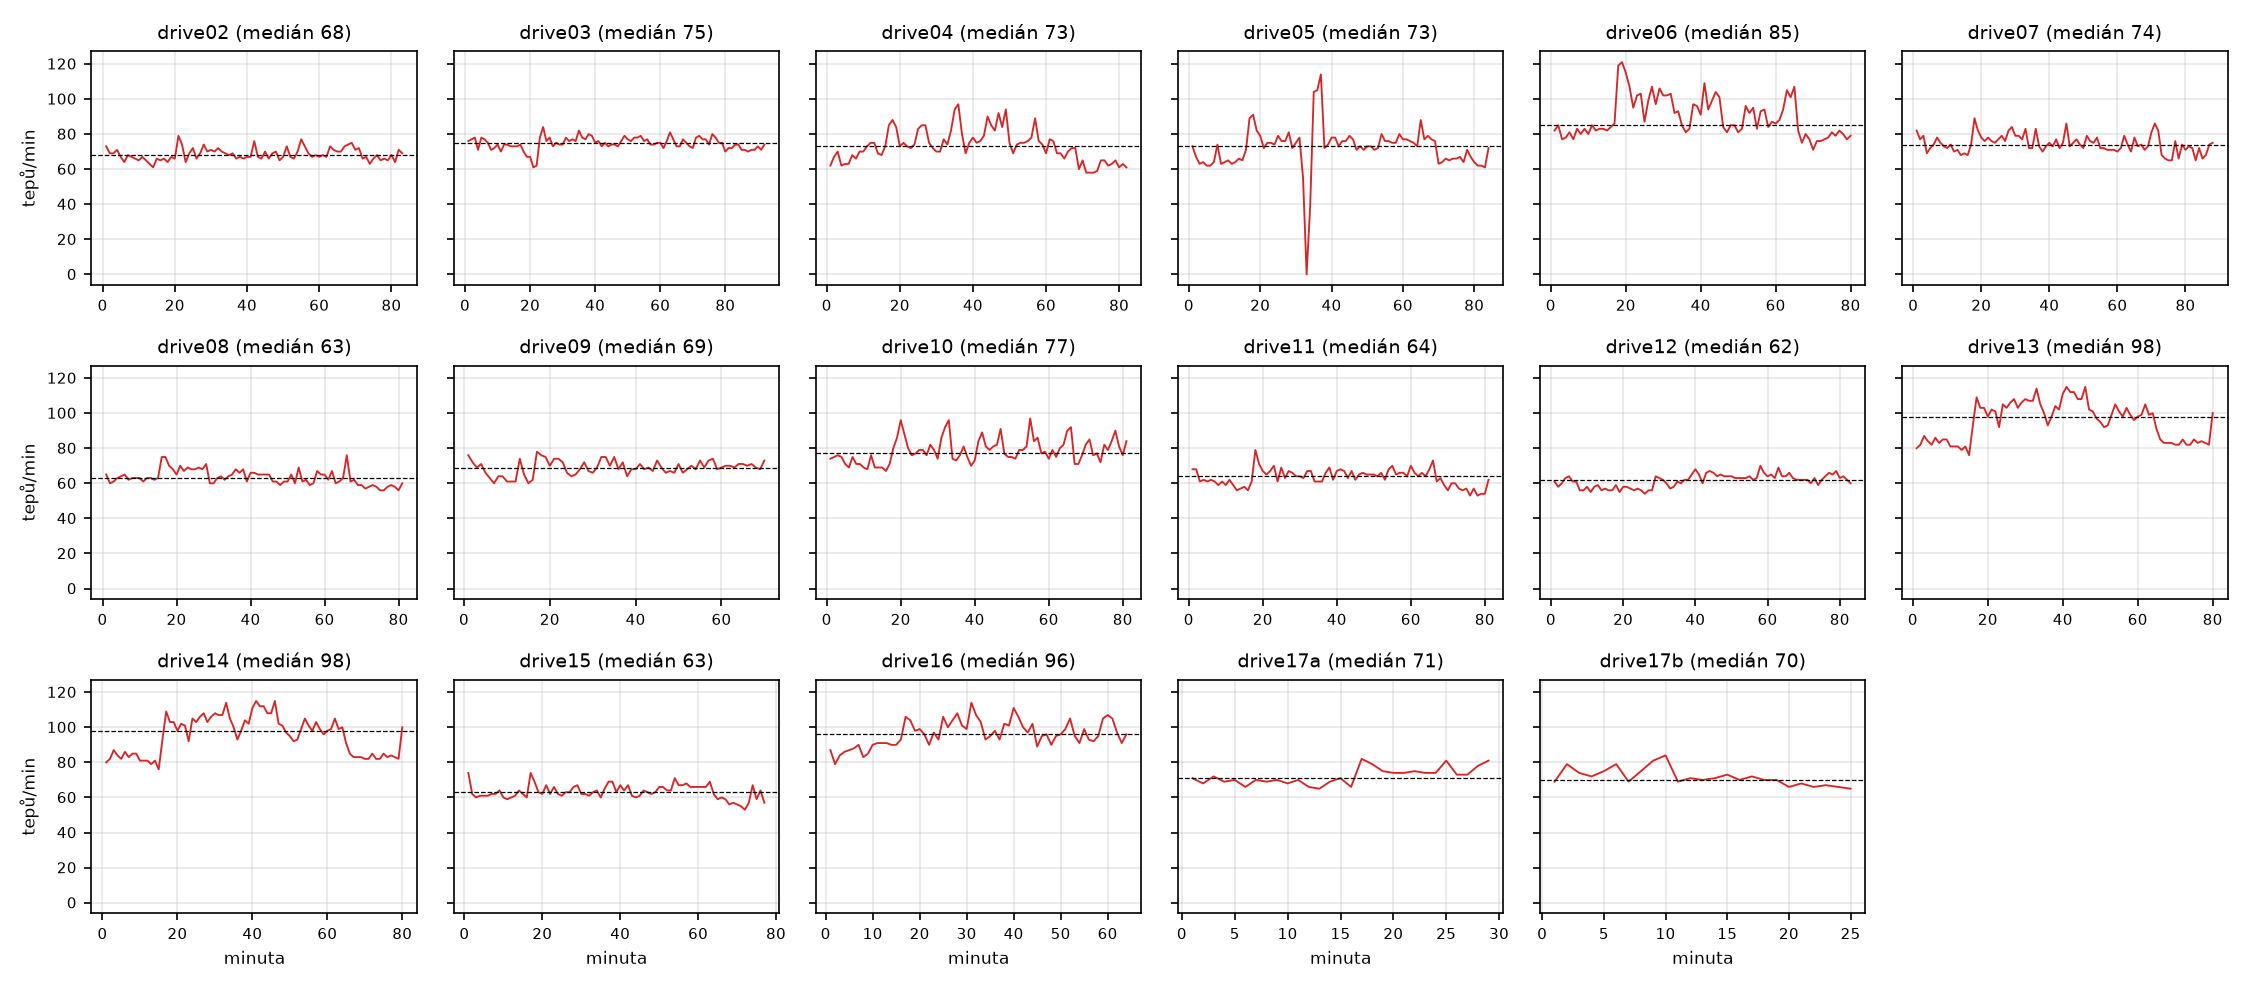
\includegraphics[width=\textwidth]{figures/drivedb_tepova_frekvence_po_minutach.png}
\caption{Počet tepů v jednotlivých minutách záznamu (\texttt{drivedb}); přerušovaná čára je
medián minutových hodnot.}
\label{fig:bpm_min}
\end{figure}

\begin{table}[H]
\centering\small
\caption{Medián, minimum a maximum minutové tepové frekvence [tepů/min] (\texttt{drivedb}).}
\label{tab:bpm_min}
\begin{tabular}{lrrr@{\hspace{1.6cm}}lrrr}
\toprule
Měření & medián & min & max & Měření & medián & min & max\\
\midrule
drive02 & 68 & 61 & 79  & drive10  & 77 & 67 & 97\\
drive03 & 75 & 61 & 84  & drive11  & 64 & 53 & 79\\
drive04 & 73 & 58 & 97  & drive12  & 62 & 54 & 70\\
drive05 & 73 & 0  & 114 & drive13  & 98 & 76 & 115\\
drive06 & 85 & 71 & 121 & drive14  & 98 & 76 & 115\\
drive07 & 74 & 65 & 89  & drive15  & 63 & 53 & 74\\
drive08 & 63 & 56 & 76  & drive16  & 96 & 79 & 114\\
drive09 & 69 & 60 & 78  & drive17a & 71 & 65 & 82\\
        &    &    &     & drive17b & 70 & 65 & 84\\
\bottomrule
\end{tabular}
\end{table}

Obrázek~\ref{fig:drive01} ukazuje detekci na začátku záznamu \texttt{drive02}. QRS komplex je
v této databázi záporný a detektor jej zachytil správně.

\begin{figure}[H]
\centering
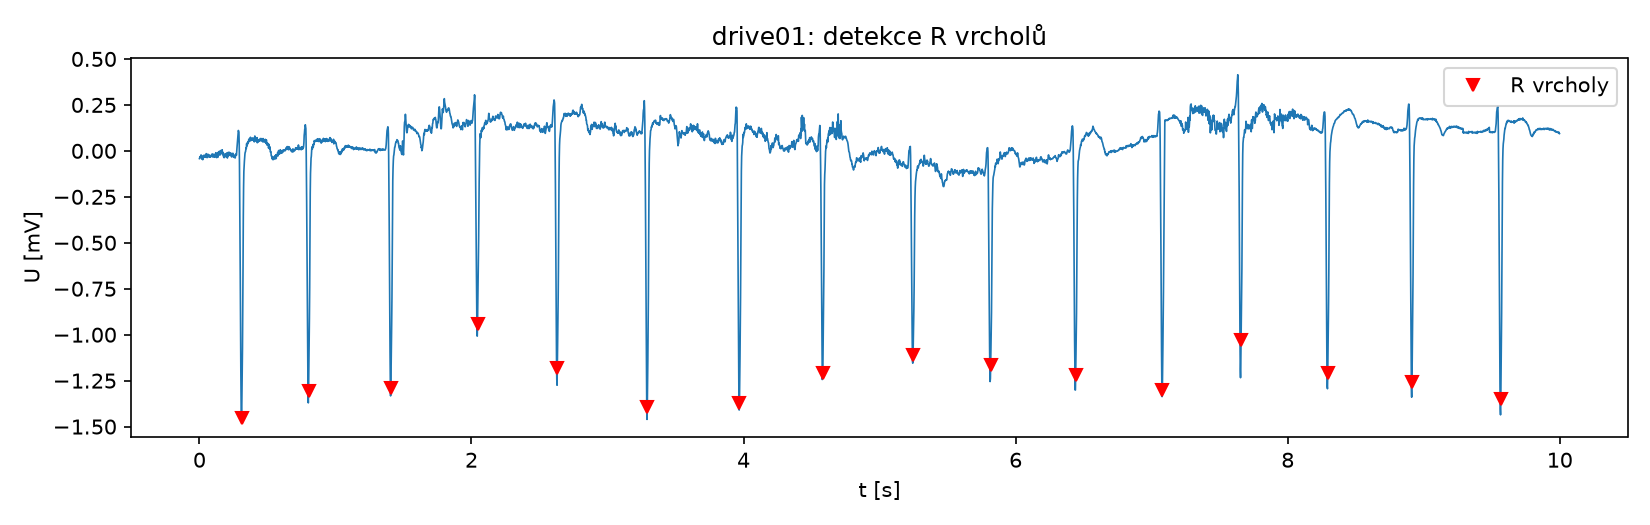
\includegraphics[width=\textwidth]{figures/drivedb_ukazka_detekce.png}
\caption{Detekce R vrcholů v prvních 10~s záznamu \texttt{drive02} (červené trojúhelníky).
         Záznam \texttt{drive01} se z PhysioNetu nepodařilo stáhnout.}
\label{fig:drive01}
\end{figure}

\paragraph{Záznam drive02.}
Původní verze detektoru našla v tomto záznamu jen 80 vrcholů (1,0~tepů/min), i když signál
je v dalších úsecích čistý (obr.~\ref{fig:drive02}). Rozsah signálu je $\pm$11,7~mV, zatímco
běžný QRS komplex má kolem 2~mV. Artefakt zvedl adaptivní práh a detektor se již nezotavil.
Po ořezu extrémních hodnot a zotavení prahu po pauze vychází 68,5~tepů/min. Stejnou
příčinu měl i záznam \texttt{drive05} (původně 63,5, nově 72,0~tepů/min).

\begin{figure}[H]
\centering
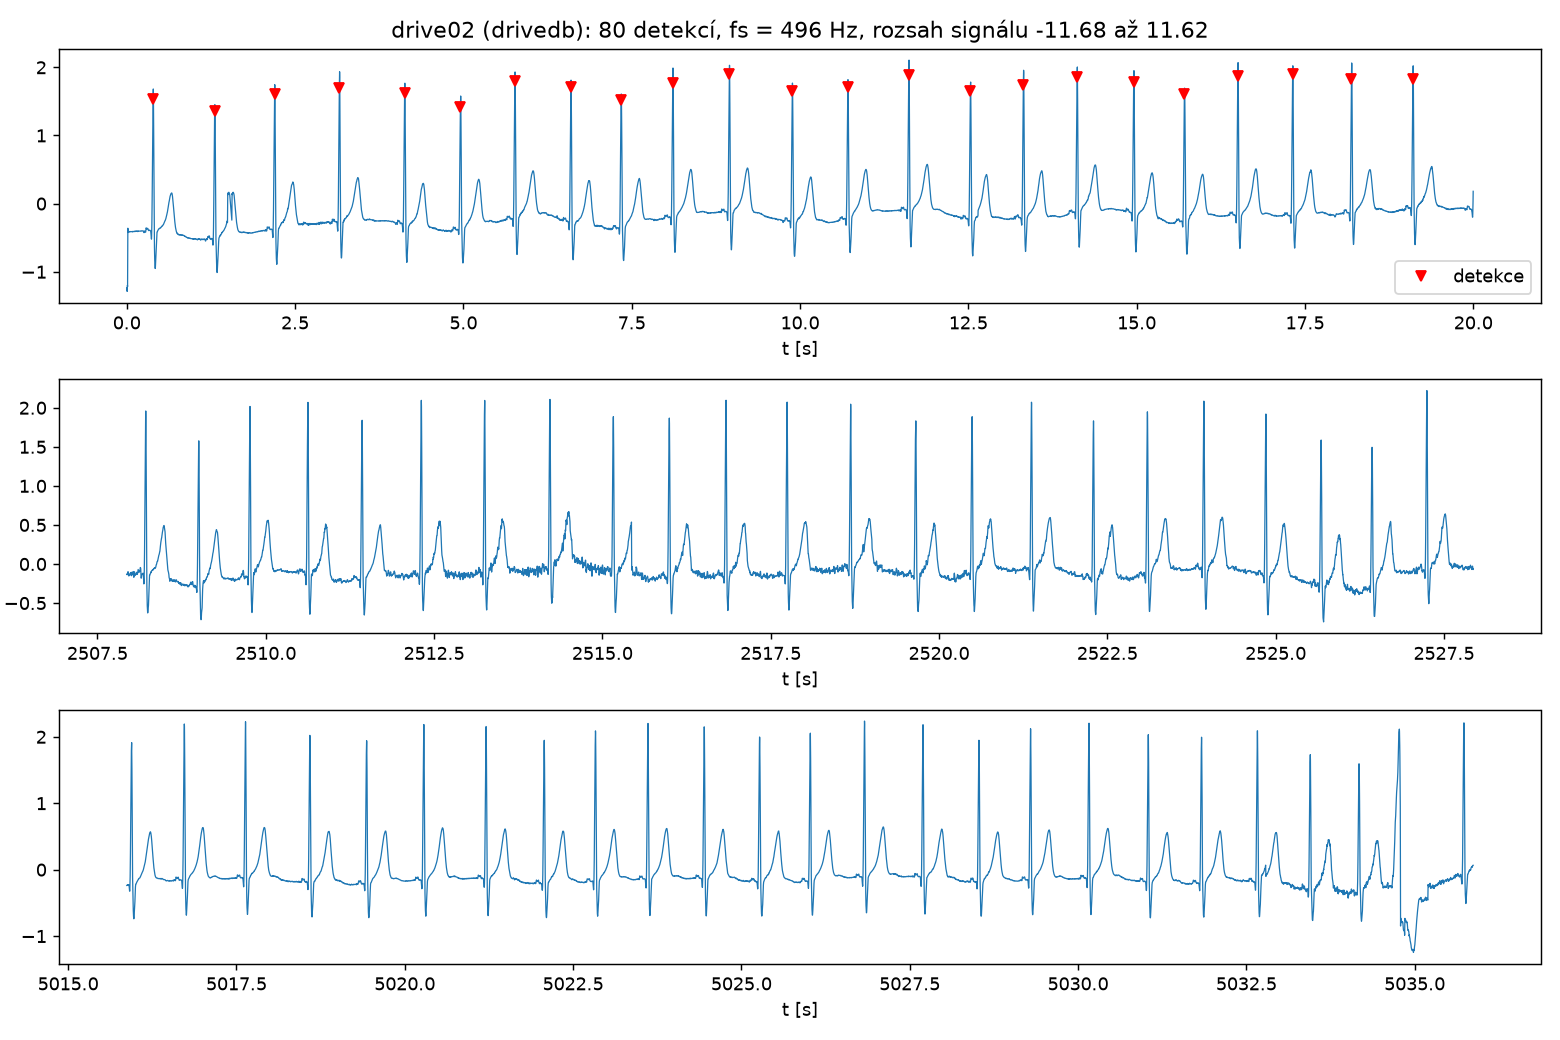
\includegraphics[width=\textwidth]{figures/ladeni_drive02_pred_upravou.png}
\caption{Záznam \texttt{drive02} před úpravou detektoru: detekce (červeně) končí po úvodním
úseku, přestože signál ve středu a na konci záznamu je čistý.}
\label{fig:drive02}
\end{figure}

\paragraph{Záznamy drive13 a drive14.}
Oba záznamy mají stejný výsledek (7665 vrcholů, 95,3~tepů/min). Hlavičky obou souborů uvádějí pro
kanál EKG shodné zesílení, počáteční hodnotu i kontrolní součet, signál EKG je tedy v obou
souborech stejný (liší se jen další kanál). Jde o vlastnost databáze, ne o chybu zpracování.

%------------------------------------------------------------------------------
\subsection{Validace na databázi \texttt{nsrdb}}
%------------------------------------------------------------------------------
Vyhodnotilo se prvních 30~minut každého z 18 záznamů (celkem 44\,263 anotovaných tepů). Detekce se
páruje s anotacemi tepů v toleranci $\pm$100~ms, což je přísnější než 150~ms doporučovaných normou
ANSI/AAMI EC57 pro hodnocení detektorů QRS: správná detekce je TP, detekce bez anotace FP,
anotace bez detekce FN.
Senzitivita je $\mathrm{TP}/(\mathrm{TP}+\mathrm{FN})$ a pozitivní prediktivní hodnota
$\mathrm{PPV}=\mathrm{TP}/(\mathrm{TP}+\mathrm{FP})$.

Detekce v neanotovaných úsecích (před první a za poslední anotací a v mezerách delších než
3~s) nelze vyhodnotit, a proto se do výsledku nepočítají. Jejich počet je ve sloupci
\emph{Vyřazeno}. Příkladem je záznam 19088 (obr.~\ref{fig:19088}): v prvním úseku nejsou
žádné anotace a signál má pilovitý tvar, v dalších úsecích detektor trefuje skutečné vrcholy.

\begin{table}[H]
\centering\footnotesize
\setlength{\tabcolsep}{4.5pt}
\caption{Úspěšnost detekce R vrcholů na databázi \texttt{nsrdb} (prvních 30 minut každého záznamu,
tolerance $\pm$100~ms). BPM ref. a BPM det. jsou počítány z vyhodnocených úseků.}
\label{tab:nsrdb}
\begin{tabular}{lrrrrrrrrrr}
\toprule
Záznam & Ref. tepy & TP & FP & FN & Se [\%] & PPV [\%] & BPM ref. & BPM det. & Vyřazeno\\
\midrule
16265 & 2751 & 2751 & 0 & 0 & 100,00 & 100,00 & 92,08 & 92,08 & 13\\
16272 & 1778 & 1778 & 7 & 0 & 100,00 & 99,61 & 64,91 & 65,16 & 167\\
16273 & 2484 & 2483 & 0 & 1 & 99,96 & 100,00 & 82,82 & 82,79 & 0\\
16420 & 2498 & 2494 & 3 & 4 & 99,84 & 99,88 & 83,29 & 83,26 & 0\\
16483 & 2754 & 2753 & 0 & 1 & 99,96 & 100,00 & 91,83 & 91,80 & 0\\
16539 & 2627 & 2627 & 1 & 0 & 100,00 & 99,96 & 87,61 & 87,64 & 0\\
16773 & 2130 & 2130 & 0 & 0 & 100,00 & 100,00 & 71,03 & 71,03 & 0\\
16786 & 2171 & 2170 & 0 & 1 & 99,95 & 100,00 & 72,41 & 72,37 & 0\\
16795 & 1911 & 1911 & 0 & 0 & 100,00 & 100,00 & 63,72 & 63,72 & 0\\
17052 & 2263 & 2263 & 0 & 0 & 100,00 & 100,00 & 75,45 & 75,45 & 0\\
17453 & 2442 & 2442 & 0 & 0 & 100,00 & 100,00 & 81,45 & 81,45 & 0\\
18177 & 3069 & 3069 & 3 & 0 & 100,00 & 99,90 & 103,31 & 103,41 & 31\\
18184 & 2621 & 2617 & 1 & 4 & 99,85 & 99,96 & 87,40 & 87,30 & 0\\
19088 & 2468 & 2468 & 0 & 0 & 100,00 & 100,00 & 99,65 & 99,65 & 602\\
19090 & 2427 & 2427 & 1 & 0 & 100,00 & 99,96 & 82,68 & 82,72 & 72\\
19093 & 2018 & 2018 & 2 & 0 & 100,00 & 99,90 & 68,31 & 68,38 & 53\\
19140 & 2707 & 2707 & 0 & 0 & 100,00 & 100,00 & 92,19 & 92,19 & 74\\
19830 & 3144 & 3143 & 0 & 1 & 99,97 & 100,00 & 106,82 & 106,79 & 63\\
\midrule
\textbf{Celkem} & \textbf{44263} & \textbf{44251} & \textbf{18} & \textbf{12} &
\textbf{99,97} & \textbf{99,96} & \textbf{83,72} & \textbf{83,73} & \textbf{1075}\\
\bottomrule
\end{tabular}
\end{table}

Celková senzitivita je 99,97~\% a PPV 99,96~\% (44\,251 správných detekcí z 44\,263 anotací,
18 falešně pozitivních a 12 falešně negativních). Průměrná absolutní chyba tepové frekvence je
0,04~tepů/min. Pokud se započítají i neanotované úseky (přepínač \texttt{--no-exclude}), vychází PPV
97,59~\% (1\,093 falešně pozitivních). Rozdíl tedy pochází téměř celý z vyřazení neanotovaných úseků
(1\,075 detekcí, z toho 602 v záznamu 19088) a nejde o zlepšení samotného algoritmu. Pro srovnání:
při vyhodnocení jen prvních 10~minut vychází Se 99,93~\% a PPV 99,90~\%.

\begin{figure}[H]
\centering
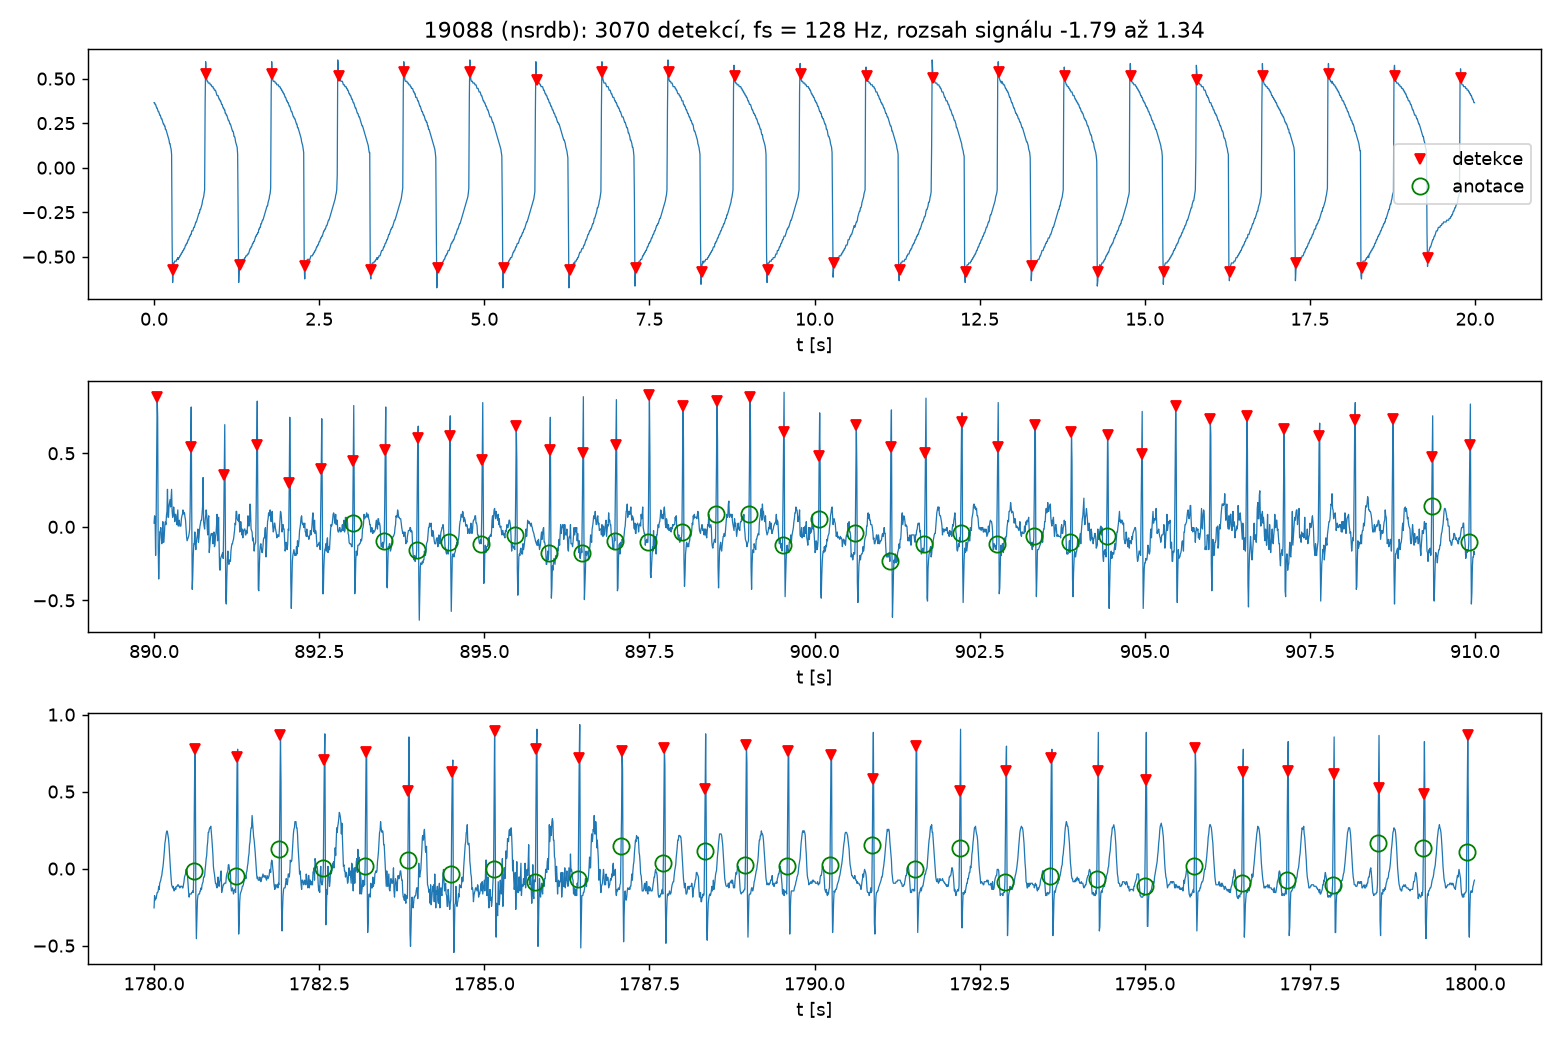
\includegraphics[width=\textwidth]{figures/ladeni_19088_pred_upravou.png}
\caption{Záznam 19088 před vyřazením neanotovaných úseků. V prvním úseku (0--20~s) nejsou
anotace, a detekce zde se tedy původně počítaly jako falešně pozitivní. Zelené kroužky
(anotace) leží několik vzorků od vrcholu R, proto je v nich signál nižší než v červených
trojúhelnících. Rozdíl pokrývá tolerance $\pm$100~ms.}
\label{fig:19088}
\end{figure}

%==============================================================================
\section{Úloha 2: Korelace signálů EKG, ABP a ICP}
%==============================================================================
\subsection{Postup řešení}
Každý signál se nejdříve sjednotí a vyčistí a teprve potom se počítají korelace, a to jak uvnitř
pacienta, tak pro ABP mezi pacienty (obr.~\ref{fig:diag-kor}).

\begin{figure}[H]
\centering
\begin{tikzpicture}[kr/.style={krok, minimum width=2.8cm, font=\footnotesize}]
  \node[popisek, anchor=west] at (-1.4,0.95) {Uvnitř pacienta: EKG, ABP, ICP};
  \node[kr] (a1) at (0,0)    {\textbf{Načtení}\\{\scriptsize 60 minut}};
  \node[kr] (a2) at (3.1,0)  {\textbf{Interpolace}\\{\scriptsize chybějící data}};
  \node[kr] (a3) at (6.2,0)  {\textbf{Ověření $f_s$}\\{\scriptsize vše 50 Hz, jinak převz.}};
  \node[kr] (a4) at (9.3,0)  {\textbf{Centralizace}\\{\scriptsize bez offsetu}};
  \node[kr, hlavni, minimum width=2.8cm] (a5) at (12.4,0) {\textbf{Korelace}\\{\scriptsize EKG, ABP, ICP}};
  \node[popisek, anchor=west] at (0.3,-1.67) {Mezi pacienty: pouze ABP};
  \node[kr] (b1) at (0,-2.7)   {\textbf{ABP}\\{\scriptsize všech 13 pacientů}};
  \node[kr] (b2) at (3.1,-2.7) {\textbf{Dominantní vrchol}\\{\scriptsize prvních 30 s}};
  \node[kr] (b3) at (6.2,-2.7) {\textbf{Zarovnání}\\{\scriptsize ořez na délku}};
  \node[kr, hlavni, minimum width=2.8cm] (b4) at (9.3,-2.7) {\textbf{Matice 13$\times$13}\\{\scriptsize celý signál}};
  \node[kr] (b5) at (12.4,-2.7) {\textbf{Matice tepů}\\{\scriptsize průměrný pulz}};
  \foreach \i/\j in {a1/a2,a2/a3,a3/a4,a4/a5,b1/b2,b2/b3,b3/b4,b4/b5}{\draw[sipka] (\i)--(\j);}
  \draw[sipka] (a4.south) -- ++(0,-0.7) -| (b1.north);
\end{tikzpicture}
\caption{Vývojový diagram výpočtu korelací. Matice tepů vychází z průměrných srdečních cyklů ABP.}
\label{fig:diag-kor}
\end{figure}

\begin{itemize}
  \item Z každého ze 13 pacientů (charis1 až charis13) se načte prvních 60~minut signálů EKG, ABP a ICP.
  \item \textbf{Vzorkovací frekvence:} podle hlaviček mají všechny tři kanály u všech 13 pacientů
        $f_s = 50$~Hz. Převzorkování (polyfázový filtr na zvolenou společnou frekvenci) proto nebylo
        nutné, kód je pro jinou $f_s$ připraven. Poté se odečte střední hodnota (centralizace).
  \item \textbf{Chybějící data:} chybějící vzorky (NaN) se doplňují lineární interpolací. V prvních
        60~minutách ale nechybí u žádného pacienta ani kanálu jediný vzorek (0~\%, viz soubor
        \texttt{kvalita\_vzorkovani\_chybejici\_data.csv}).
  \item Uvnitř pacienta se pro dvojice EKG--ABP, EKG--ICP a ABP--ICP počítá Pearsonův koeficient
        $r$ bez zpoždění a maximum normované vzájemné korelace $r_{\max}$ pro zpoždění $\tau$
        v rozsahu $\pm$0,5~s (výpočet přes FFT). Kladné $\tau$ znamená, že druhý signál zaostává
        za prvním. Okno je kratší než jeden srdeční cyklus záměrně: u periodických signálů se
        maximum při delším okně může posunout o celý tep a zpoždění pak nemá fyziologický význam
        (s oknem $\pm$2~s vycházelo např. $\tau = -2{,}00$~s na samém okraji okna).
  \item Mezi pacienty se ABP zarovná na první dominantní systolický vrchol (první vrchol v prvních
        30~s s výškou alespoň na úrovni 75. percentilu), ořízne se na stejnou délku a spočítá
        se matice $13\times 13$ Pearsonových koeficientů. Navíc se porovnávají průměrné srdeční
        cykly (100 bodů), které nejsou zkreslené rozdílnou tepovou frekvencí pacientů.
\end{itemize}

%------------------------------------------------------------------------------
\subsection{Výsledky}
%------------------------------------------------------------------------------
\paragraph{Korelace signálů uvnitř pacienta.}
Obrázek~\ref{fig:kor-pac} a tabulka~\ref{tab:kor} ukazují shodu signálů u jednotlivých pacientů.
ABP a ICP spolu jasně korelují jen u části pacientů, zatímco EKG s tlakovými signály korelují
prakticky vůbec.

\begin{figure}[H]
\centering
\begin{tikzpicture}
\begin{axis}[
  ybar, bar width=4.2pt, width=\textwidth, height=6.5cm,
  xmin=0.4, xmax=13.6, ymin=-0.5, ymax=1,
  xtick={1,...,13}, xticklabels={1,...,13},
  ytick={-0.5,0,0.5,1}, yticklabels={$-0{,}5$,0,0{,}5,1},
  xlabel={Pacient (charis\textit{n})}, ylabel={Pearsonův koeficient $r$},
  ymajorgrids, grid style={black!12},
  extra y ticks=0, extra y tick style={grid=major, grid style={black!60}, tick label style={font=\footnotesize}},
  legend style={at={(0.5,1.03)}, anchor=south, legend columns=3, font=\footnotesize, draw=none,
                /tikz/every even column/.append style={column sep=0.4cm}},
  legend image code/.code={\draw[#1, draw=none] (0cm,-0.1cm) rectangle (0.25cm,0.15cm);},
  tick label style={font=\footnotesize}, label style={font=\small}, axis line style={black!60}
]
\addplot[fill=black!55, draw=black!55] coordinates {
 (1,0.031) (2,-0.098) (3,-0.089) (4,0.024) (5,0.024) (6,-0.403) (7,-0.086)
 (8,0.127) (9,0.071) (10,0.301) (11,0.298) (12,-0.015) (13,0.025)};
\addplot[fill=black!22, draw=black!35] coordinates {
 (1,0.075) (2,-0.082) (3,-0.147) (4,-0.113) (5,0.030) (6,-0.357) (7,-0.084)
 (8,-0.042) (9,0.028) (10,-0.023) (11,0.251) (12,0.004) (13,-0.006)};
\addplot[fill=blue!70!black, draw=blue!70!black] coordinates {
 (1,-0.019) (2,0.496) (3,0.849) (4,0.014) (5,0.002) (6,0.521) (7,0.616)
 (8,0.326) (9,0.281) (10,0.532) (11,0.614) (12,0.306) (13,0.030)};
\legend{EKG--ABP, EKG--ICP, ABP--ICP}
\end{axis}
\end{tikzpicture}
\caption{Korelační koeficient $r$ (zpoždění 0) mezi signály jednotlivých pacientů.}
\label{fig:kor-pac}
\end{figure}

\begin{table}[H]
\centering\footnotesize
\setlength{\tabcolsep}{4pt}
\caption{Pearsonův koeficient $r$ (zpoždění 0) a maximum vzájemné korelace $r_{\max}$ v okně $\pm$0,5~s
(v závorce zpoždění $\tau$ v sekundách). Žádné maximum neleží na okraji okna.}
\label{tab:kor}
\begin{tabular}{lrrrrrr}
\toprule
 & \multicolumn{2}{c}{EKG--ABP} & \multicolumn{2}{c}{EKG--ICP} & \multicolumn{2}{c}{ABP--ICP}\\
Pacient & $r$ & $r_{\max}$ ($\tau$) & $r$ & $r_{\max}$ ($\tau$) & $r$ & $r_{\max}$ ($\tau$)\\
\midrule
charis1  & 0,031 & \m0,032 (0,02)  & 0,075 & \m0,165 (0,26)  & \m0,019 & \m0,027 (\m0,34)\\
charis2  & \m0,098 & 0,388 (0,28)  & \m0,082 & \m0,188 (0,12) & 0,496 & 0,529 (\m0,02)\\
charis3  & \m0,089 & \m0,212 (0,10) & \m0,147 & \m0,252 (0,08) & 0,849 & 0,849 (0,00)\\
charis4  & 0,024 & \m0,032 (0,02)  & \m0,113 & 0,156 (0,46)    & 0,014 & 0,025 (0,48)\\
charis5  & 0,024 & 0,024 (0,00)    & 0,030 & \m0,105 (0,12)  & 0,002 & 0,005 (\m0,28)\\
charis6  & \m0,403 & 0,566 (0,26)  & \m0,357 & \m0,555 (0,10) & 0,521 & 0,546 (0,02)\\
charis7  & \m0,086 & 0,325 (0,30)  & \m0,084 & 0,204 (0,32)   & 0,616 & 0,630 (\m0,02)\\
charis8  & 0,127 & \m0,271 (\m0,12) & \m0,042 & \m0,164 (\m0,18) & 0,326 & 0,343 (\m0,04)\\
charis9  & 0,071 & 0,143 (0,06)    & 0,028 & 0,084 (0,10)    & 0,281 & 0,364 (0,06)\\
charis10 & 0,301 & \m0,386 (\m0,20) & \m0,023 & \m0,466 (\m0,16) & 0,532 & 0,719 (0,08)\\
charis11 & 0,298 & 0,396 (0,06)    & 0,251 & 0,263 (0,02)    & 0,614 & 0,639 (\m0,02)\\
charis12 & \m0,015 & \m0,106 (0,16) & 0,004 & 0,004 (0,00)   & 0,306 & 0,306 (\m0,08)\\
charis13 & 0,025 & 0,165 (0,22)    & \m0,006 & \m0,021 (\m0,48) & 0,030 & 0,040 (0,06)\\
\bottomrule
\end{tabular}
\end{table}

Nejsilnější vztah mají ABP a ICP: u pacientů charis2, 3, 6, 7, 10 a 11 je $r$ kolem 0,5 až 0,85
(nejvíce 0,85 u charis3) a maximum vzájemné korelace leží blízko nulového zpoždění. U charis1, 4 a 5
je korelace ABP--ICP nulová. EKG s tlakovými signály nekoreluje, nejvýraznější hodnoty jsou
$-0{,}40$ (EKG--ABP) a $-0{,}36$ (EKG--ICP) u charis6. To je očekávané, protože EKG je elektrický
signál a tlakové křivky mají jiný tvar i časování, takže jejich okamžitá lineární shoda je slabá.

\paragraph{Korelace ABP mezi pacienty.}
Obrázky~\ref{fig:heatmapa} a~\ref{fig:heatmapa-tep} zobrazují matice $13\times 13$ korelačních
koeficientů ABP po zarovnání na dominantní vrchol, nejdříve pro celý signál, potom pro průměrný
srdeční cyklus. Číselné hodnoty matice průměrných cyklů uvádí tabulka~\ref{tab:abp-tep}.

\begin{figure}[H]
\centering
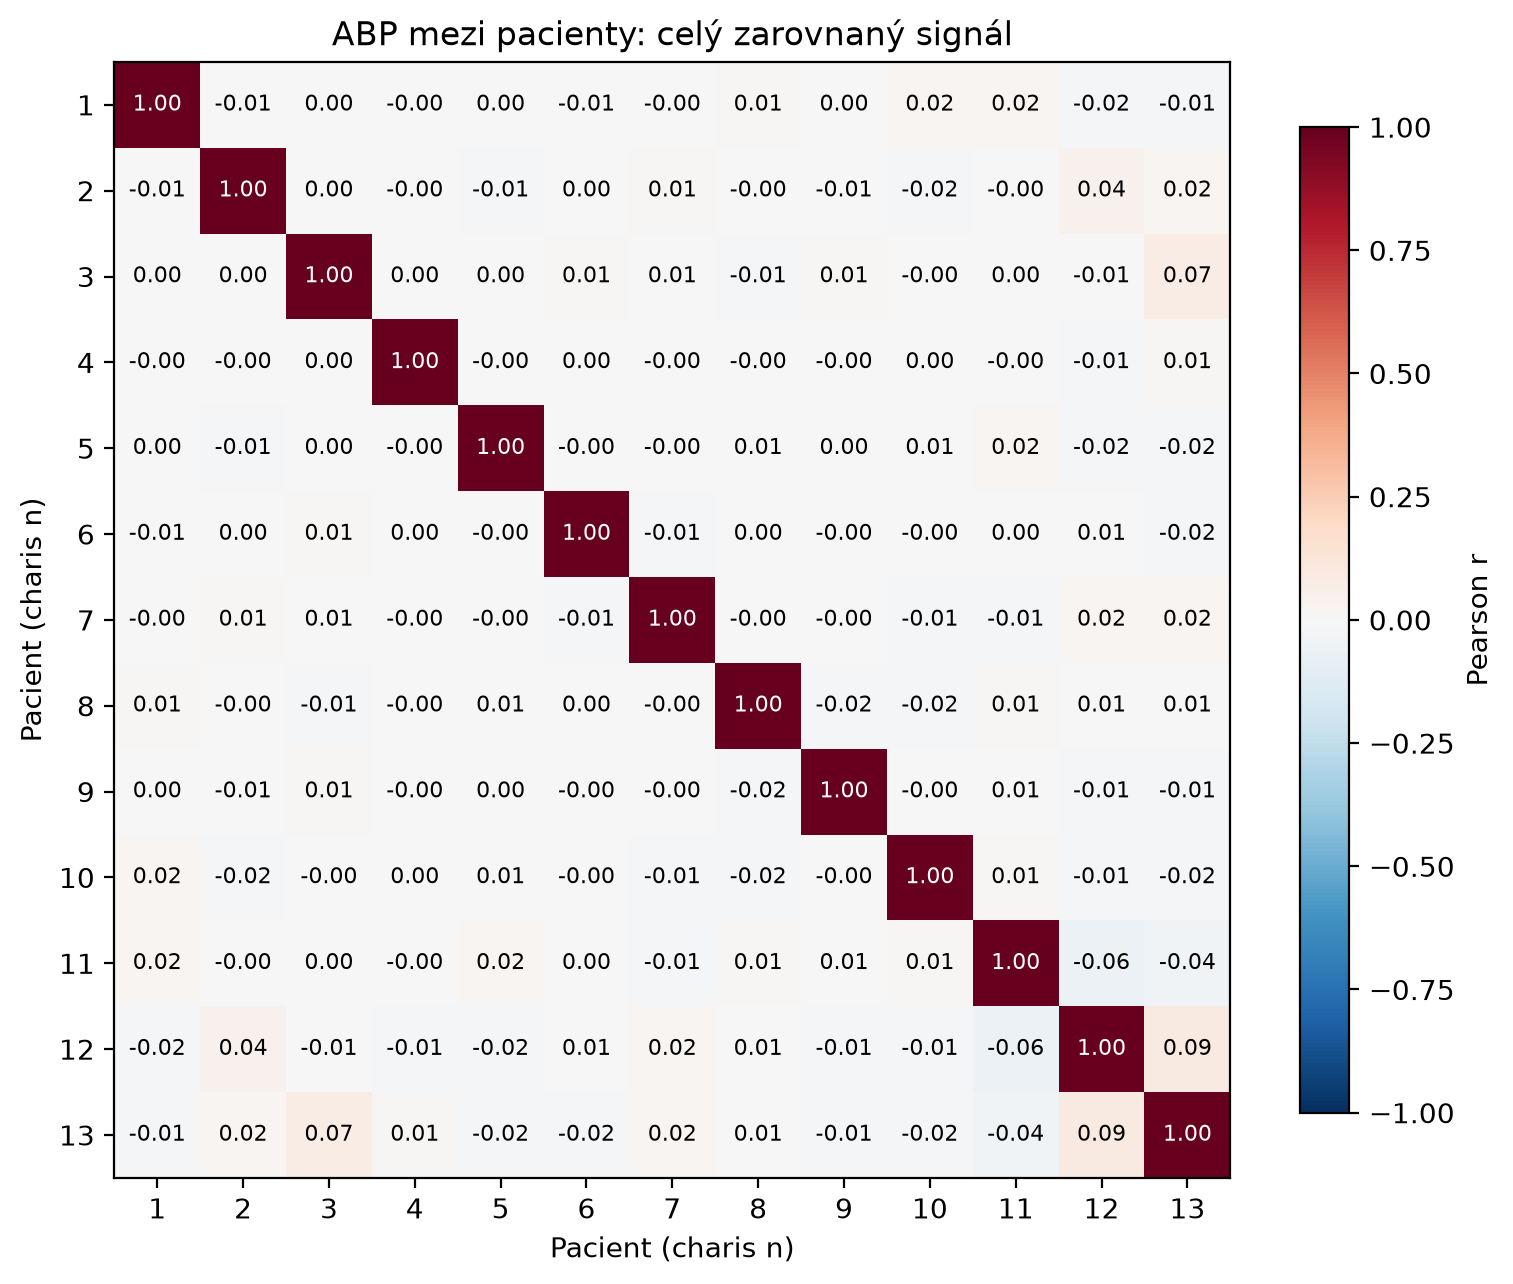
\includegraphics[width=0.78\textwidth]{figures/korelace_ABP_mapa_cely_signal.png}
\caption{Korelace ABP mezi pacienty: celý zarovnaný signál (60~minut).}
\label{fig:heatmapa}
\end{figure}

\begin{figure}[H]
\centering
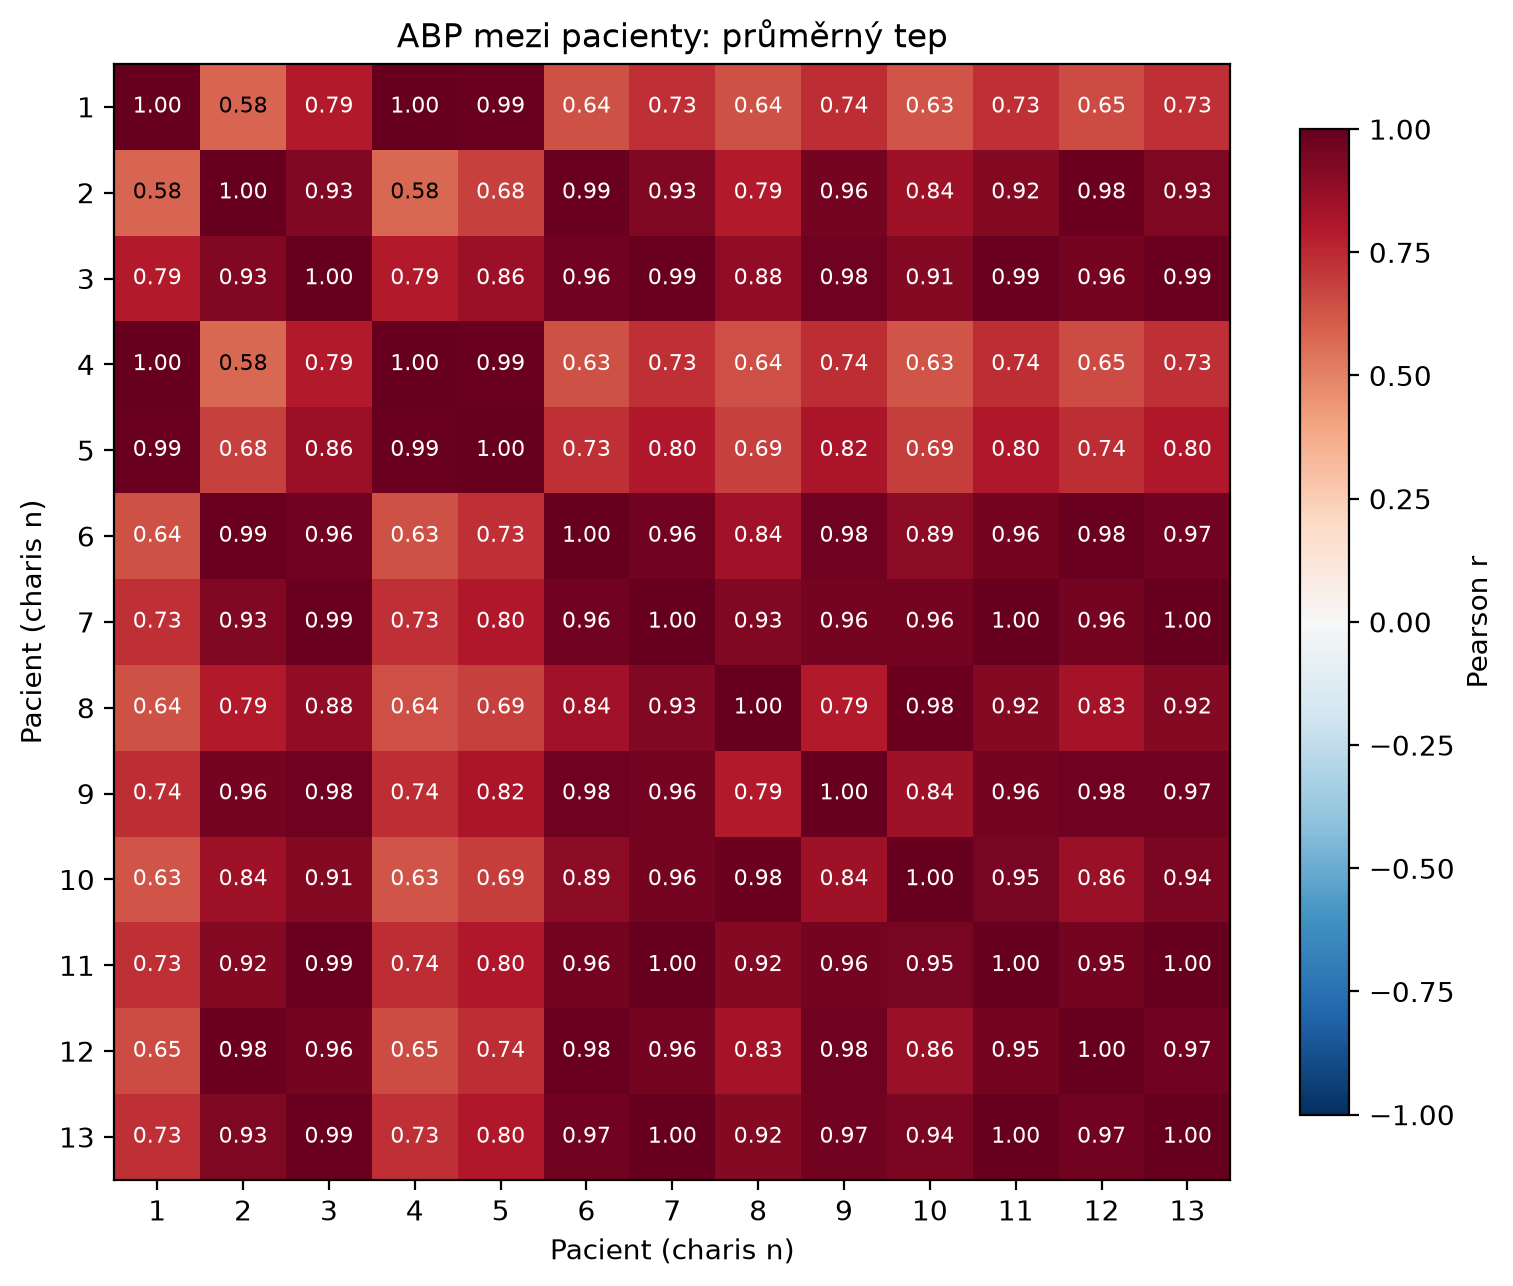
\includegraphics[width=0.78\textwidth]{figures/korelace_ABP_mapa_prumerny_tep.png}
\caption{Korelace ABP mezi pacienty: průměrný srdeční cyklus (100 bodů na tep).}
\label{fig:heatmapa-tep}
\end{figure}

\begin{table}[H]
\centering\footnotesize
\setlength{\tabcolsep}{3.5pt}
\caption{Pearsonův koeficient $r$ mezi průměrnými srdečními cykly ABP pacientů charis\textit{n}
(matice je symetrická, uveden je dolní trojúhelník). Hodnoty pro celý signál jsou v souboru
\texttt{korelace\_ABP\_mezi\_pacienty.csv}, všechny leží v intervalu $|r| < 0{,}1$.}
\label{tab:abp-tep}
\begin{tabular}{r*{12}{c}}
\toprule
n & 1 & 2 & 3 & 4 & 5 & 6 & 7 & 8 & 9 & 10 & 11 & 12\\
\midrule
2 & 0,58 &  &  &  &  &  &  &  &  &  &  & \\
3 & 0,79 & 0,93 &  &  &  &  &  &  &  &  &  & \\
4 & 1,00 & 0,58 & 0,79 &  &  &  &  &  &  &  &  & \\
5 & 0,99 & 0,68 & 0,86 & 0,99 &  &  &  &  &  &  &  & \\
6 & 0,64 & 0,99 & 0,96 & 0,63 & 0,73 &  &  &  &  &  &  & \\
7 & 0,73 & 0,93 & 0,99 & 0,73 & 0,80 & 0,96 &  &  &  &  &  & \\
8 & 0,64 & 0,79 & 0,88 & 0,64 & 0,69 & 0,84 & 0,93 &  &  &  &  & \\
9 & 0,74 & 0,96 & 0,98 & 0,74 & 0,82 & 0,98 & 0,96 & 0,79 &  &  &  & \\
10 & 0,63 & 0,84 & 0,91 & 0,63 & 0,69 & 0,89 & 0,96 & 0,98 & 0,84 &  &  & \\
11 & 0,73 & 0,92 & 0,99 & 0,74 & 0,80 & 0,96 & 1,00 & 0,92 & 0,96 & 0,95 &  & \\
12 & 0,65 & 0,98 & 0,96 & 0,65 & 0,74 & 0,98 & 0,96 & 0,83 & 0,98 & 0,86 & 0,95 & \\
13 & 0,73 & 0,93 & 0,99 & 0,73 & 0,80 & 0,97 & 1,00 & 0,92 & 0,97 & 0,94 & 1,00 & 0,97\\
\bottomrule
\end{tabular}
\end{table}

Při porovnání celých zarovnaných signálů vychází každá dvojice pacientů s $|r|<0{,}1$ (nejvíce 0,09 u charis12 a charis13), tedy bez vztahu. To je očekávané: zarovnání na první dominantní vrchol sjednotí jen začátek a při různé tepové frekvenci se fáze srdečních cyklů během hodiny rozejdou. Levá matice proto o podobnosti pulzové křivky nic nevypovídá. Matice průměrných srdečních cyklů, která je na tepovou frekvenci necitlivá, ukazuje vysokou podobnost tvaru pulzu: mezi deseti pacienty (charis2, 3, 6 až 13) je nejnižší hodnota 0,79 a řada dvojic dosahuje 1,00 (např. charis7, 11 a 13). Výjimkou jsou pacienti charis1, 4 a 5, kteří spolu korelují 0,99 až 1,00, ale s ostatními jen 0,58 až 0,86. Stejní tři pacienti mají nulovou korelaci ABP s ICP (tab.~\ref{tab:kor}), proto je pravděpodobné, že jejich ABP má jiný tvar nebo horší kvalitu. K potvrzení by bylo třeba záznamy prohlédnout.

%==============================================================================
\section{Zhodnocení a závěr}
%==============================================================================
Detektor R vrcholů dosáhl na databázi \texttt{nsrdb} senzitivity 99,97~\% a PPV 99,96~\%.
Korelace potvrdily souvislost jen mezi signály ABP a ICP.

\begin{itemize}
  \item \textbf{Úloha 1.} Algoritmus Pan--Tompkins s ořezem artefaktů a zotavením prahu našel
        44\,251 z 44\,263 referenčních tepů (18 falešně pozitivních), průměrná absolutní chyba
        tepové frekvence je 0,04~tepů/min. V \texttt{drivedb} vychází tepová frekvence 61,5 až
        96,2~tepů/min.
  \item \textbf{Omezení úlohy 1.} PPV se počítá jen v anotovaných úsecích: vyřazeno bylo 1\,075 detekcí
        (2,4~\%), bez vyřazení je PPV 97,59~\%. Test proběhl na prvních 30~minutách každého
        záznamu \texttt{nsrdb} (záznamy mají přibližně 24~h). Pro \texttt{drivedb} nemáme referenční anotace, správnost se proto
        ověřila jen nepřímo na \texttt{nsrdb} a vizuálně. Záznam \texttt{drive14} má stejné EKG
        jako \texttt{drive13}.
  \item \textbf{Úloha 2.} ABP a ICP korelují s $r$ od 0,5 do 0,85 u šesti ze 13 pacientů (charis2, 3,
        6, 7, 10 a 11), u charis1, 4, 5 a 13 je $|r|$ pod 0,04. U dobře korelovaných dvojic leží
        maximum blízko nulového posunu ($|\tau|\le 0{,}08$~s). EKG s tlakovými signály nekoreluje:
        u sedmi pacientů z 13 je $|r|$ pod 0,1 pro EKG--ABP i EKG--ICP a nejvyšší hodnota je
        0,40 (charis6, EKG--ABP). Elektrický signál EKG a tlakové signály ABP a ICP se při nulovém
        posunu tvarem nepodobají, nulová korelace proto neznamená, že spolu nesouvisejí.
        Z toho důvodu je u každé dvojice uvedeno i maximum vzájemné korelace se zpožděním.
\end{itemize}

%==============================================================================
\begin{thebibliography}{9}
\bibitem{physionet} Goldberger, A. L. et al.: PhysioBank, PhysioToolkit, and PhysioNet.
  \emph{Circulation}, 101(23):e215--e220, 2000.
\bibitem{pantompkins} Pan, J., Tompkins, W. J.: A Real-Time QRS Detection Algorithm.
  \emph{IEEE Transactions on Biomedical Engineering}, BME-32(3):230--236, 1985.
\bibitem{drivedb} Healey, J. A., Picard, R. W.: Detecting Stress During Real-World Driving Tasks
  Using Physiological Sensors. \emph{IEEE Transactions on Intelligent Transportation Systems},
  6(2):156--166, 2005. Databáze: \url{https://physionet.org/content/drivedb/1.0.0/}.
\bibitem{charisdb} Kim, N. et al.: Trending autoregulatory indices during treatment for traumatic
  brain injury. \emph{Journal of Clinical Monitoring and Computing}, 30(6):821--831, 2016.
  Databáze: \url{https://physionet.org/content/charisdb/1.0.0/}.
\bibitem{scipy} Virtanen, P. et al.: SciPy 1.0: fundamental algorithms for scientific computing
  in Python. \emph{Nature Methods}, 17:261--272, 2020.
\end{thebibliography}

\end{document}
